\documentclass{article}

\usepackage[T1]{fontenc} 
\usepackage[utf8]{inputenc}
\usepackage[francais]{babel}
\usepackage{graphicx}


\title{Rendu EDD strategie}
\author{Pinero, Borde, Bonnet}

\begin{document}
\maketitle
\tableofcontents

\newpage
\section{Strategie fonctionnelle}
La strategie fonctionnelle choisie pour le rapport est la stratégie du coin. Pour cela, nous avions fait un premier algorithme qui se contente de jouer vers la gauche tant qu'on le peut, sinon il joue vers le bas encore une fois tant qu'on le peut, de même vers la droite puis vers le haut. Avec cet stratégie, sur 48 parties nous avons un score moyen de 2475, avec 6x64, 20x128, 20x256 et 2x512.

Dans un seconds temps, nous avons fait un second algorithme qui est basé sur le premier mais qui un coups sur deux change les mouvements favoris. Les premiers mouvements favoris sont dans cet ordre, gauche, bas, droite et haut, et les seconds mouvements sont dans cet ordre, bas, gauche, droite et haut. Avec cet stratégie, sur 48 parties nous avons un score moyen de 2259, avec 1x32, 3x64, 21x128 et 23x256.

Les deux stratégies se valent à peu prés, mais c'est bien la première qui est la meilleure.

\section{La libraire dynamique}
La libraire A2\_bonnet\_borde\_pinero\_basic.so est g\'en\'er\'ee dans le r\'epertoire \og lib/ \fg{}. Cette librairie implemente l'interface \og include/strategy.h \fg{}. Elle contient une m\'ethode appel\'ee {\itshape A2\_bonnet\_borde\_pinero\_basic()} et qui retourne la strategie.

\clearpage
\section{Evaluation de la grille}
\label{eval_grid}
Pour évaluer la grille, nous avons pris en compte quatre paramèrtres, et à chancun de ces paramètres nous leurs avons donné un coéficient pour leurs donner plus ou moins d'importance. 


	\subsection{Le nombre de tile vide}
	On compte le nombre de tile vide que l'on a après avoir joué et on le mutiplie par
	\subsection{La plus grande tile} 
	Est la valeur de la tile avec la plus grande valeur.

	\subsection{La grille la plus progressive possible}
	Une grille est progressive lorsque la valeur des cases augmente ou descende quelle que soit la direction. Ainsi, 2 - 4 - 8 - 16 est acceptable, tout comme 32 - 8 - 4 - 2. Mais 2 - 8 - 2 - 16 ne l'est pas (\`a cause de la 3eme case). \`A chaque mouvement on doit verifier si  le mouvement d'apr\`es rendra la grille plus progressive. Si c'est le cas, le mouvement doit \^etre effectu\'e. Si non, trouver un autre mouvement.

	\subsection{La grille la plus réguli\`ere possible}
	pour pouvoir fusionner, les cases doivent comporter des valeurs identiques. Ainsi une suite 2 - 16 - 64 - 256 respecte la r\`egle de progressivit\`e) mais aboutira à un \'echec car on ne pourra fusionner aucune case avec sa voisine. Il faut donc respecter un autre crit\`ere : la r\'egularit\'e. Et faire en sorte de ne pas avoir de cassure dans les s\'eries. Entre cr\'eer une série 2 - 4 - 8 - 16 et cr\'eer une s\'erie 16 - 64 - 256 - 1024 on pr\'ef\'erera donc la premi\`ere, m\^eme si la possibilit\'e d'obtenir un nombre fort comme 1024 peut \^etre tentante a priori.

\clearpage
\section{Reflexion avanc\'e sur l'implementation de expected max}
\og Expected Max \fg{} est un algorithme qui consiste \`a retourner la direction optimale \`a jouer. Elle est bas\'ee sur l'algorithme \og minimax \fg{}. Le principe est de donner une valeure à la grille en fonction de plusieurs critères (cf. \og \ref{eval_grid} Evaluation de la grille \fg{}) ainsi nous jouerons le coups avec le maximum de chance de gagné combiné au coup avec le minimum de chance de perdre. Ici nous avons un exemple avec le morpion :

\begin{figure}[!h]
   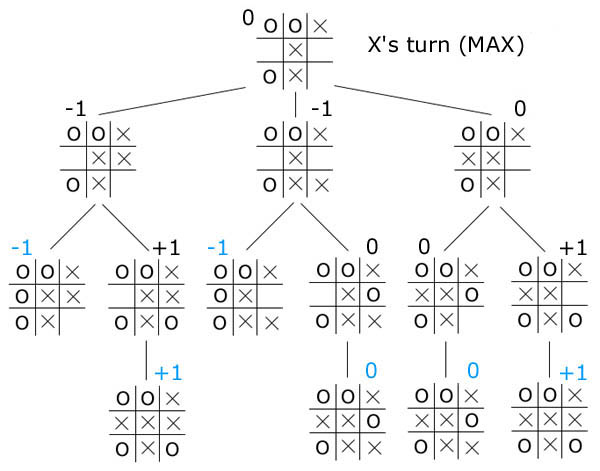
\includegraphics[width=7cm,height=7cm]{minimax.jpg}
   \caption{\label{minimax} Exemple minimax}
\end{figure}

Dans la figure 1, on peut voir que le coups le plus interessant à jouer est le troisi\`eme, car si on fait la somme de chaque branche de l'arbre (-2, 1, -2, -1, 0, 2), c'est celle-ci qui offre le plus grand score et la perte la moins importante.

L'une des limites de cette m\'ethode est qu'il faille jouer \`a deux joueurs, or au 2048 on joue tout seul. C'est pour cette raison qu'on utilisera pas le th\'ehor\`eme du \og minimax \fg{} mais celui d'\og Expected Max \fg{}. En effet ici on concid\`erera le second joueur comme l'ordinateur qui remplira de façon aléatoire une des tiles vides. Cela engage de calculer, pour chaque grille et pour toutes les possibilit\'es de remplissage d'une tile vide, la valeur de cette grille. Il faudra ensuite faire une moyenne de toutes les valeurs calculés afin de déterminer quel chemin est le plus interressent. Pour un algorithme encore plus performant il serait avantageux de pouvoir \'etendre notre arbre \`a une profondeur N choisi au d\'ebut du programme. Il parait évident qu'une telle technique va avoir un cout en mémoire et calcule important. Hors dans la mesure ou des limitations en temps d'éxcution nous sont imposé il faudra trouver un équilibre entre résultats et performances.

\end{document}